\documentclass[letter,11pt]{article}
\usepackage[margin=1.5cm]{geometry}
\usepackage{latexsym}
\usepackage{amsmath}
\usepackage{color}
\usepackage{graphicx}
\usepackage{amssymb}
\usepackage{alltt}
\usepackage{enumitem}
\usepackage{siunitx}
\usepackage{physics}
\usepackage{float}
\usepackage{bm}
\usepackage{hyperref}

\newenvironment{solution}{
    \vspace{0.16in} {\bf Solution:}
    
}{
	\vspace{0.16in}
}

\DeclareMathOperator*{\argmax}{arg\,max}
\DeclareMathOperator*{\argmin}{arg\,min}

\newcommand{\xx}{\bm{x}}
\newcommand{\vv}{\bm{v}}
\newcommand{\T}{T}
\newcommand{\RR}{\mathbb{R}}
\newcommand{\mub}{\bm{\mu}}
\newcommand{\thetab}{\bm{\theta}}
\newcommand{\Sigmab}{\bm{\Sigma}}
\newcommand{\m}[1]{\begin{bmatrix}#1\end{bmatrix}}
\newcommand{\N}{\mathcal{N}}
\newcommand{\PP}{\mathbb{P}}
\newcommand{\Dc}{\mathcal{D}}
\newcommand{\Nc}{\mathcal{N}}
\newcommand{\ww}{\mathbf{w}}
\newcommand{\0}{\mathbf{0}}
\newcommand{\yy}{\mathbf{y}}

%------------------------------------------------------

\begin{document}

\begin{center}
    {\bf \Large Math 189R problem set 8} \\
    \vspace{0.1in}
    Adam Guo \quad 2020-04-13
\end{center}

\begin{enumerate}
    \item \textbf{(K-means)} In this problem, we will implement the k-means algorithm and separate 5,000 2D data points into different number of clusters.
    
    Let $X = {x_1, x_2 \ldots, x_m} $ be the data points, and let $k$ be the number of clusters. The k-means algorithm is summarized as following:

    \begin{enumerate}
        \item Randomly initialize $k$ cluster centers, $\mu_1, \mu_2 \ldots \mu_k$, in the feature space.
        \item Calculate the distance between each data points and the cluster centers.
        \item Assign each data point to the cluster center $c$ whose distance between this data point is the minimum of all the cluster centers, namely, \[c_i = \argmin_j ||x_i - \mu_j||^2\]
        \item Update each cluster center to be \[\mu_j = \frac{\sum_{i=1}^{m}1\{c_i = j\}x_i}{\sum_{i = 1}^{m}1\{c_i = j\}}\]
        \item Repeat step 2 - 4 until convergence or exhausted.
    \end{enumerate}

    The objective (cost) function is defined as \[J(c, \mu) = \sum_{i = 1}^{m}||x_i - \mu_{c_i}||^2\]
    
    In this assignment, you will first implement the k-means cost function and the algorithm. Then, for $k = 1, 2 \ldots, 20$, find the number of clusters with the optimal cost and produce a plot of the relationship between the cost and the number of clusters. Then, visualize the data points and the cluster centers on the optimal number of clusters.
    
    Notice that the k-means algorithm might yield different results based on the randomness of the initialization of cluster centers.

    \begin{solution}
        \begin{figure}[H]
            \centering
            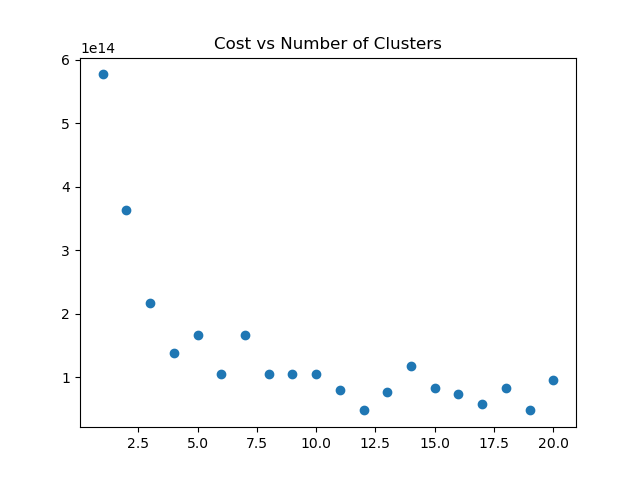
\includegraphics[width=10cm]{kmeans_1.png}
            \caption{Plot of cost vs. number of clusters}
        \end{figure}

        \begin{figure}[H]
            \centering
            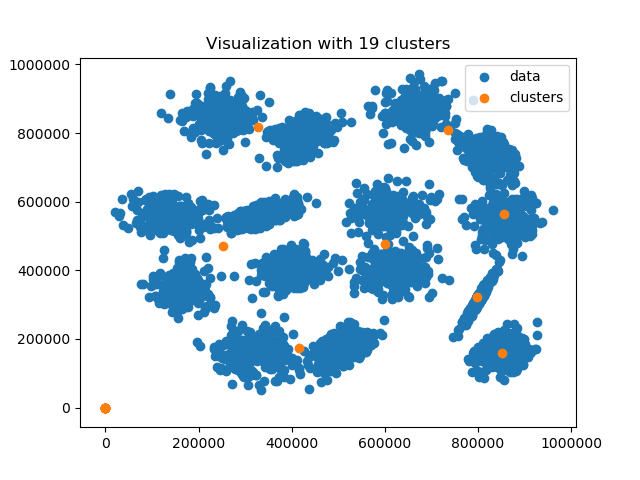
\includegraphics[width=10cm]{kmeans_2.png}
            \caption{Plot of points and clusters}
        \end{figure}
    \end{solution}

    \newpage

    %----------------------------------

    \item \textbf{Extra Credit (Non-Negative Matrix Factorization)}
    
    In this problem, we will use the reuters dataset in nltk library. Please run nltk.download() in python shell to download the dataset. In the starter code, we have already parsed the data for you.
    
    Choosing an appropriate objective function and algorithm from Lee and Seung 2001 \footnote{\url{https://papers.nips.cc/paper/1861-algorithms-for-non-negative-matrix-factorization.pdf}} implement Non-Negative Matrix Factorization for topic modelling (choose an appropriate number of topics/latent features) and assert that the convergence properties proved in the paper hold. Display the 20 most relevant words for each of the topics you discover.

    \begin{solution}
        \begin{figure}[H]
            \centering
            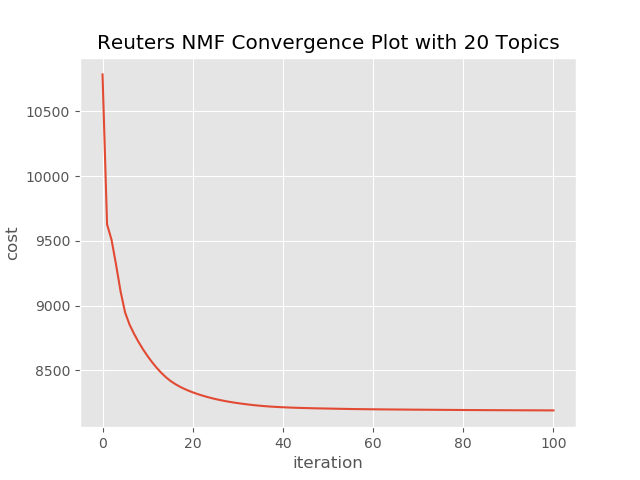
\includegraphics[width=10cm]{nmf_cvg.png}
            \caption{NMF convergence plot}
        \end{figure}

        \begin{figure}[H]
            \centering
            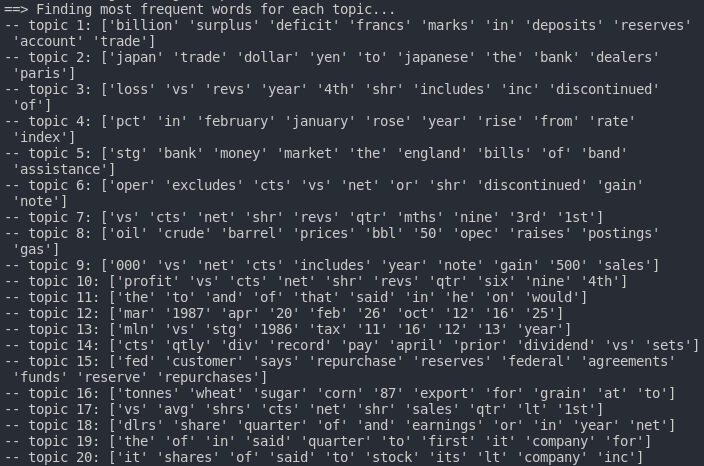
\includegraphics[width=12cm]{q2.png}
            \caption{Most common words in each topic}
        \end{figure}
    \end{solution}

    % \newpage

    % %----------------------------------

    % \item \textbf{Extra Credit (Linear Regression)} Consider the Bayesian Linear Regression model with the following generative process:
    
    % \begin{enumerate}
    %     \item Draw $\ww \sim \Nc(\0, \mathbf{V}_0)$
    %     \item Draw $\yy_i \sim \Nc(\ww^\T\xx_i, \sigma^2)$ for $i=1,2,\dots,n$ where $\sigma^2$ is known.
    % \end{enumerate}

    % Express this model as a directed graphical model using Plate notation. Is $\yy_i$ independent of $\ww$? Is $\yy_i$ independent of $\ww$ \textit{given} $\Dc = \{\xx_i\}$? Support these claims.
\end{enumerate}

\end{document}